\clearpage
\section{Performance Analysis}\label{section:performance_analysis}

The first prototype of the new AFE was delivered for analysis right after it was assembled, meaning that even the hardware team didn't have any valid data about its performance at the time. Once it was up and running it was put to testing to assess its suitability for the upcoming pulse oximetry designs.

\subsection{Testing the Prototype's Receiver with Static Signals}

DC signals were used to measure the static performance of the system. This allowed measuring the amplifying, sampling and conversion noise without the effect of distortion and/or ringing possibly induced by a dynamic signal. The measurements were done with different setups, including one with a standard sensor, one without a cable and one with nothing connected to the board.

In effect, only a zero input signal was used for a simple reason: most of the low frequency noise of the signal chain is removed when subtracting ambient from the signal, which means that a non-zero DC signal would either still result in zero output because of the ``ambient'' removal or be incomparable because of unremoved low frequency noise.

The measurements were done as a set of series, varying one parameter in each. Figures \ref{fig:rx_noise_vs_gain} and \ref{fig:rx_noise_vs_pulse_length} show the most important results: The performance proved to be acceptable with low gains but not good enough with higher ones, the target being a standard deviation of 13 LSB or less. Figure \ref{fig:rx_noise_vs_pulse_length} proved that shot noise originating from the photodetector is not significant as increasing sampling time and thus effectively decreasing the system's bandwidth has no significant effect on the total noise. As the $R_f$ dependent noise was dominating it was suggested that the differential amplifier selected by the hardware team might not be ideal for this chip.

The theory prompted a test to see what was the actual quality of the input signal. For that, two special cases of measurement setups were built: one with a sensor head soldered right into the connector and encased in tinfoil eliminating all possible interference caused by the sensor cable, and one without anything at all connected to the board. Figure \ref{fig:cable_effect} shows the differences of the setups -- it can easily be seen that noise in input (which shows as $R_f$-dependent) is increased when the cable is attached, disturbing the measurement when using higher gains. The increase in noise is due to electrical interference induced in the cable, and it was concluded that the $R_f$-dependent noise was mostly external rather than caused by the chip itself.

Figure \ref{fig:rx_noise_vs_pulse_length} also proves that the chip has some properties ideal for low-power use: the settling times of the receiver chain are low which means that pulse length isn't an important factor in the total performance, enabling very short pulses and thus small duty ratios.

\begin{figure}[htcb]
\begin{center}
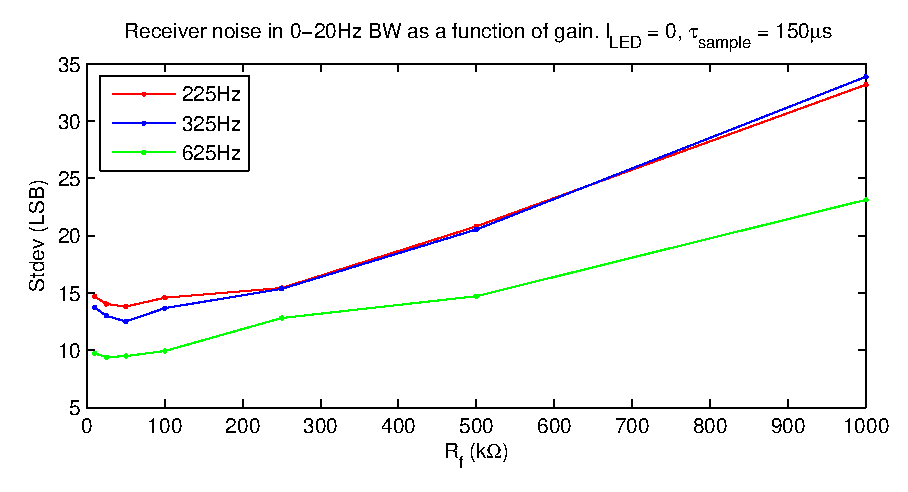
\includegraphics{kuvat/measurements/rx_noise_vs_gain.eps}
\caption{Receiver noise as a function of gain with several pulse repetition frequencies. The results are analogous to the theoretical model in figure \ref{fig:receiver_noise_model}, showing a constant and an $R_f$ dependent noise component. Also it can be seen that the performance is better with a higher pulse repetition frequency.}
\label{fig:rx_noise_vs_gain}
\end{center}
\end{figure}

\begin{figure}[htcb]
\begin{center}
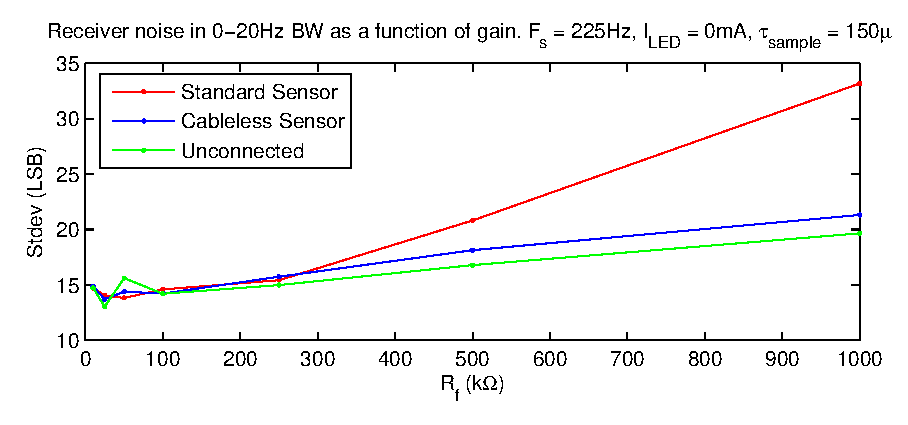
\includegraphics[scale=1]{kuvat/measurements/cable_effect.eps}
\caption{The effect of cable and sensor on receiver noise.}
\label{fig:cable_effect}
\end{center}
\end{figure}

\begin{figure}[htcb]
\begin{center}
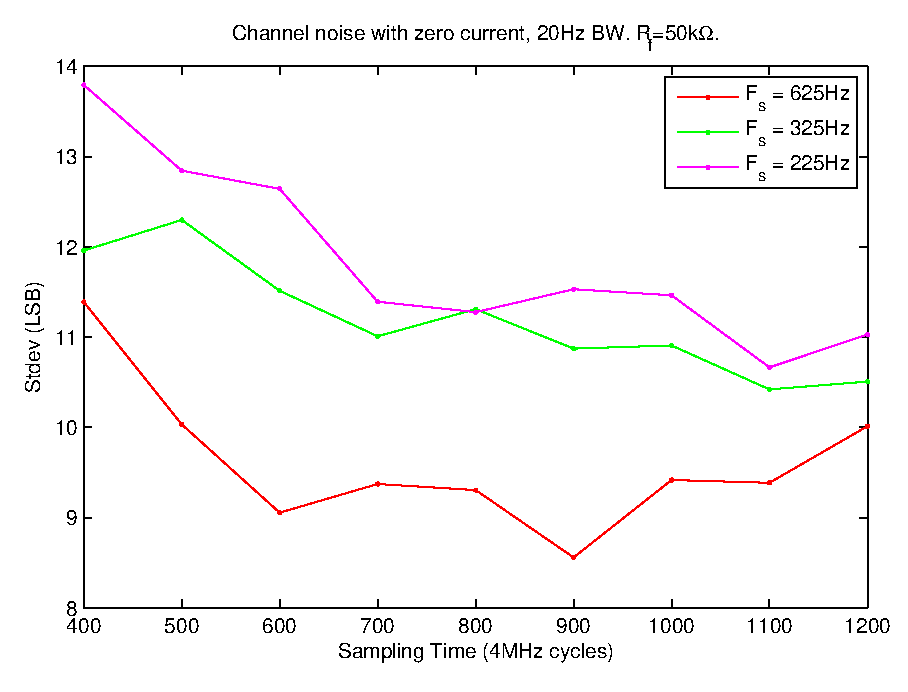
\includegraphics[scale=0.8]{kuvat/measurements/rx_noise_vs_pulse_length.eps}
\caption{Receiver noise as a function of pulse width with several pulse repetition frequencies. The results show that above a certain lower limit increasing the width of the sampling window doesn't significantly affect the receiver's performance.}
\label{fig:rx_noise_vs_pulse_length}
\end{center}
\end{figure}

Figure \ref{fig:rx_noise_vs_gain} also indicates that using a higher pulse repetition frequency has a positive effect on the performance, as expected, since decimating the signal to the target output frequency allows for filtering and averaging. An important notion is that the system's settling times are independent of sampling frequency, meaning that the same pulse width can be maintained regardless of PRF, resulting in the fact that lower PRF means a lower duty ratio and therefore lower power consumption -- clearly indicating a trade-off between performance and low power usage.

\subsection{Testing the Transmitter Only}

The transmitter was tested with a test setup shown in figure \ref{fig:tx_dc_test_setup}, the point being to provide the receiver with a zero-mean signal that had all the transmitter's noise. Assuming RMS behavior, it was possible to estimate the noise behavior of the transmitter when outputting a DC signal. Figure \ref{fig:tx_dc_noise} shows that the transmitter's signal-to-noise ratio is rather constant and high (115 dB), proving that the receiver is the system's bottleneck. It's to be noted that there's a bit more noise when using a combination of diodes and a resistor as the load -- this is natural since with the diodes in place there's a constant additional voltage drop, meaning that the system has to be driven with a larger voltage throughout the current scale.

\begin{figure}[htcb]
\begin{center}
  \input{kuvat/tx_dc_test_setup_2.eps_tex}
  \caption{The test setup of the transmitter using DC current. The circuit eliminates the DC part and passes only the AC signal, i.e. transmitter noise. The 20 $\Omega$ resistor can be replaced with a number of diodes and a smaller resistor to simulate the voltage-current response of an actual sensor.}
  \label{fig:tx_dc_test_setup}
\end{center}
\end{figure}

\begin{figure}[htcb]
\begin{center}
	\input{kuvat/measurements/noise_vs_dc_current.eps_tex}
  \caption{The calculated transmitter noise as a function of current, measured using the test setup in figure \ref{fig:tx_dc_test_setup}.}
  \label{fig:tx_dc_noise}
\end{center}
\end{figure}

The transmitter was also tested for its linearity using a standard sensor. It had to be done with a pulsed signal as a DC current of more than 50 mA would probably have burned the sensor during the test. Current linearity is important since with a well-behaving transmitter it's easier to adapt to changing conditions without disturbing the \spo algorithm. Figure \ref{fig:current_linearity} shows the relationship between the LED current setting and the measurement, and it can be seen that it is very linear. Only with added resistance does the curve stray from the optimum, mostly due to limited drive voltage.

\begin{figure}[cb]
  \begin{center}
    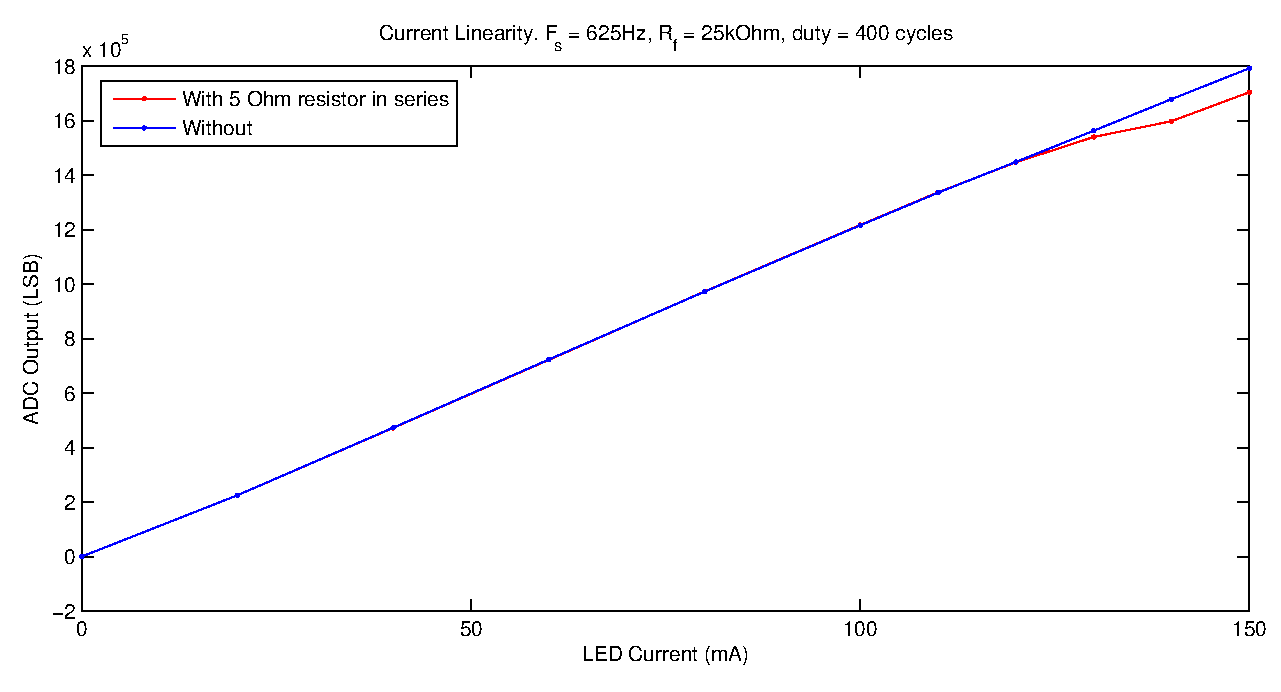
\includegraphics[scale=0.7]{kuvat/measurements/current_linearity.eps}
    \caption{The linearity of the transmitter with normal measurement configuration and with added resistance. Nonlinearity with high currents and an added resistance is due to limited drive voltage.}
    \label{fig:current_linearity}
  \end{center}
\end{figure}

\subsection{Testing the Prototype with Pulsed Signals}

The testing of the system's dynamic properties was begun by measuring system noise with different pulsed LED currents and continued by measuring system noise with a constant pulsed LED current as a function of receiver gain. The tests show that the system's performance drops significantly when a pulsed LED current is introduced in the equation (figure \ref{fig:noise_vs_current}), suggesting that there's something wrong with the dynamic properties of either the receiver or the transmitter. To resolve the root cause, the transmitter was measured alone with an external ADC and was found to behave well throughout the current range, leaving the receiver as the only option. Also the spectral power distribution of the system noise was examined to locate the band of interest.

\begin{figure}[htcb]
  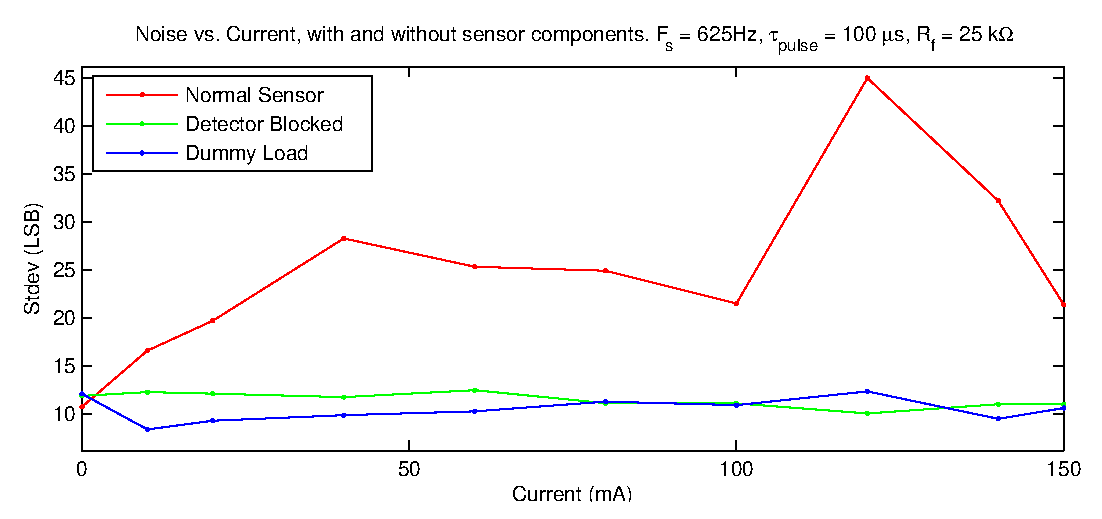
\includegraphics[scale=0.8]{kuvat/measurements/noise_vs_current.eps}
  \caption{System noise as a function of LED current. It can be seen that system performance drops significantly once LED current is introduced, indicating that the dynamic properties of either the receiver or the transmitter are below specification.}
  \label{fig:noise_vs_current}
\end{figure}

\subsubsection{Crosstalk Between the Transmitter and the Receiver}

As the noise of the system increased as a function of transmitter current it was hypothesized that there might be some unwanted crosstalk between the transmitter and the receiver. Their coupling through other paths than through the LED-photodetector interface was tested by blocking the photodetector completely and measuring the signal and system noise with different current settings. With this test it was possible to conclude if the transmitter signal would affect the measurement through some coupling on the board on in the cable. Figure \ref{fig:tx_rx_crosstalk} shows that there's no notable effect of this sort.

\begin{figure}[htcb]
\begin{center}
  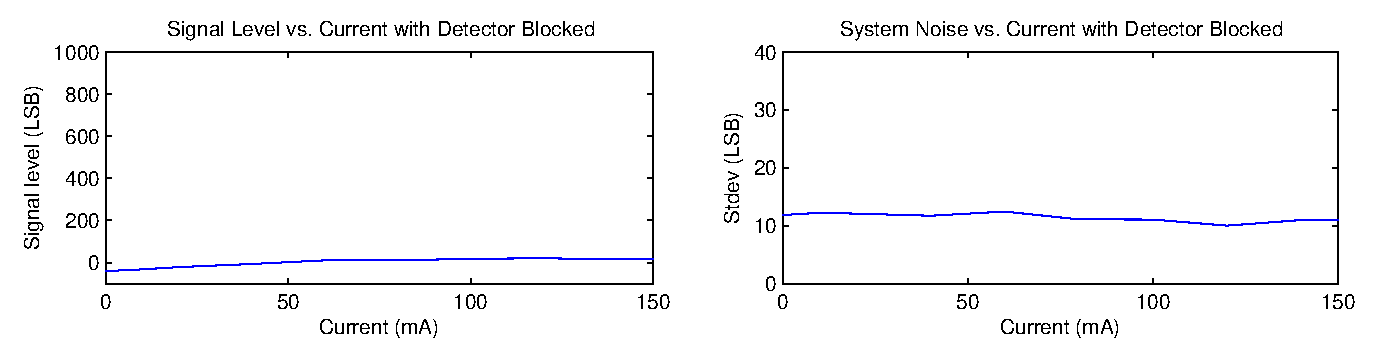
\includegraphics[scale=0.65]{kuvat/measurements/tx_rx_crosstalk.eps}
  \caption{Signal level and system noise as a function of LED current when the photodetector is blocked. Conclusion: no significant crosstalk between the transmitter and the receiver.}
  \label{fig:tx_rx_crosstalk}
\end{center}
\end{figure}

\subsubsection{Ambient Subtraction and Noise Correlation}

Crosstalk didn't provide any new insight to the performance problem so the matter was investigated further. From previous measurements it especially stood out that the ambient subtraction didn't seem to perform optimally, leaving low frequency noise in the output signal. The evaluation software was modified to allow examining the individual ambient and channel measurements separately instead of just looking at the final, subtracted signal, and an interesting phenomenon was discovered: the correlation of the noises in the signals decreased as the channel signal level increased, making system noise reduction by ambient subtraction less efficient.

As the transmitter had already been ruled out as the noise source, it was concluded that the noise properties of some component in the receiver chain depended either on the amplitude of the continuous, pulsed signal or the DC levels of the sampled signals. Figure \ref{fig:red_ambient_correlation} visualizes the correlation of the noises in the red and the red ambient channels as a function of signal level, showing that even at zero signal the correlation is below 70\%. This narrowed the focus to the receiver chain after the amplifier, mainly the sampling and conversion circuits. Figure \ref{fig:red_vs_ambient_noise} on the other hand shows the result of low correlation of the channels: as the signal level in the red channel is increased its noise increases as well while the noise of the ambient channel remains relatively constant, and as a result the noise advantage gained from subtracting the two signals becomes smaller and smaller.

\begin{figure}[htcbp!]
\begin{center}
	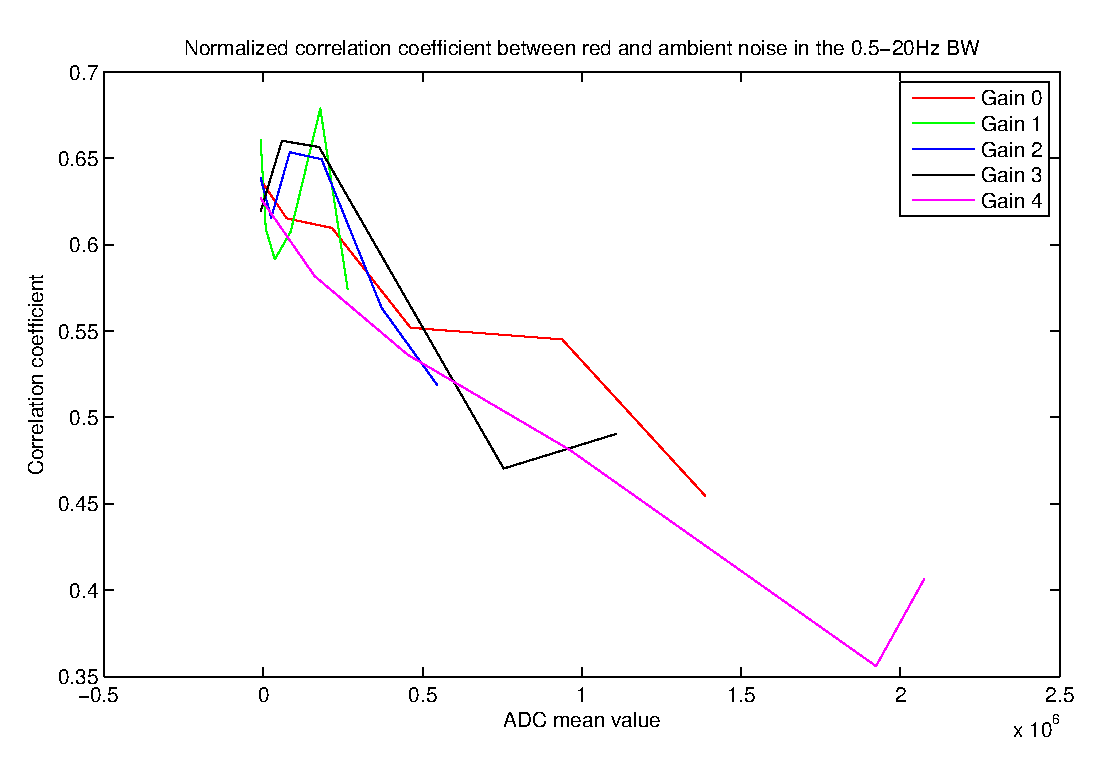
\includegraphics[scale=0.7]{kuvat/measurements/red_ambient_correlation.eps}
	\caption{The correlation of the red signal noise and the corresponding ambient signal noise in the target bandwidth as a function of signal level. The graph shows that as signal level grows the correlation decreases, indicating a noise source that only affects one of the signals.}
	\label{fig:red_ambient_correlation}
\end{center}
\end{figure}

\begin{figure}[htcbp!]
\begin{center}
  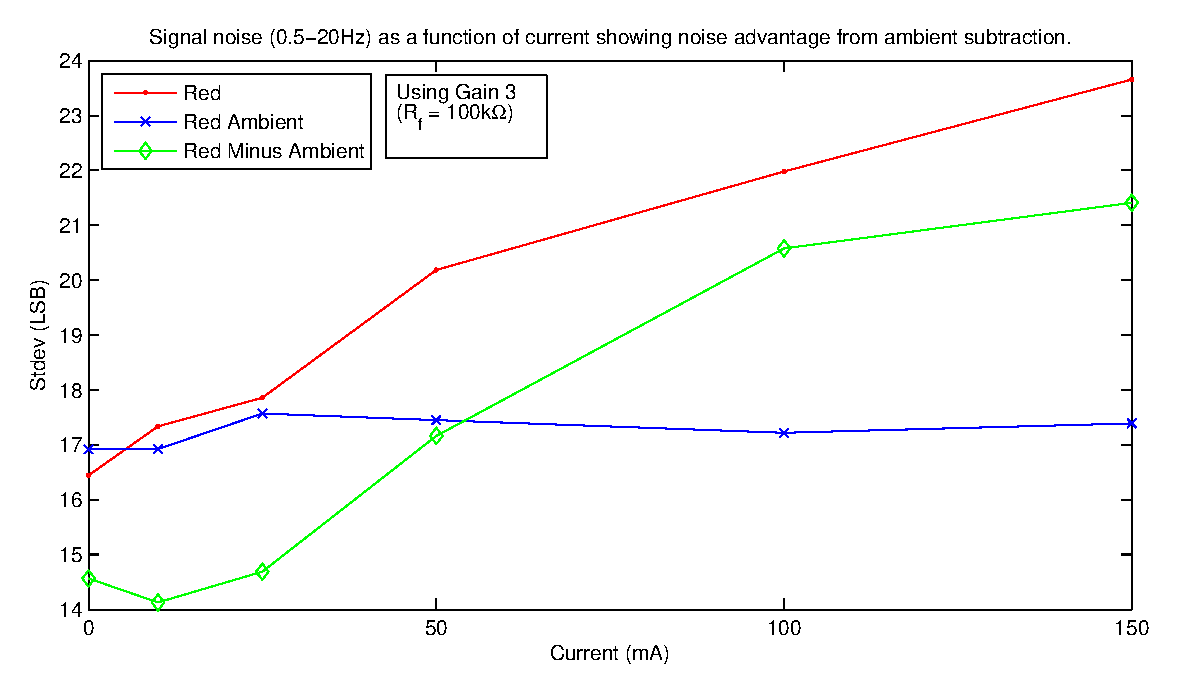
\includegraphics[scale=0.7]{kuvat/measurements/red_vs_ambient_noise.eps}
  \caption{The noises of the red and red ambient signals and also the noise of the signal resulting from subtracting the latter from the former. The graph shows that as signal level increases the efficiency of noise reduction by subtraction drops. This is due to decreased correlation between the channels as indicated in figure \ref{fig:red_ambient_correlation}.}
  \label{fig:red_vs_ambient_noise}
\end{center}
\end{figure}

From a signal processing perspective, the whole content of the ambient channel is noise that doesn't bear any valuable information but only disturbs the measurement, and therefore should be completely removed from the information-carrying signal. On the other hand, the noise in the channels has two components: one that has a common source and therefore correlates, and one that doesn't. In signal subtraction the correlated noise is diminished and the uncorrelated one increased, meaning that the noise minimum is reached by using a scaling factor between zero and one for the ambient that depends on the ratio of correlated and uncorrelated noise. As figure \ref{fig:red_vs_ambient_noise} showed that the absolute noise level of the ambient channel is rather constant throughout the signal scale, the conformity of the curves in figure \ref{fig:noise_vs_ambient_scaling} indicates that only the uncorrelated noise increases in the signal channel when signal level is increased. It would suggest that something in or after the sample-and-hold circuits has a signal level dependent noise behavior.

Increasing sampling time was not found to improve the situation after a certain minimum value so the focus was shifted to the ADC and its buffer. As the ADC is a precision part capable of much higher sample rates than with which it is used in the application studied, the quality of the buffer circuitry was questioned. At this point the data gathered was turned over to the hardware team for them to study.

%\begin{figure}[htcb!]
%\begin{center}
%  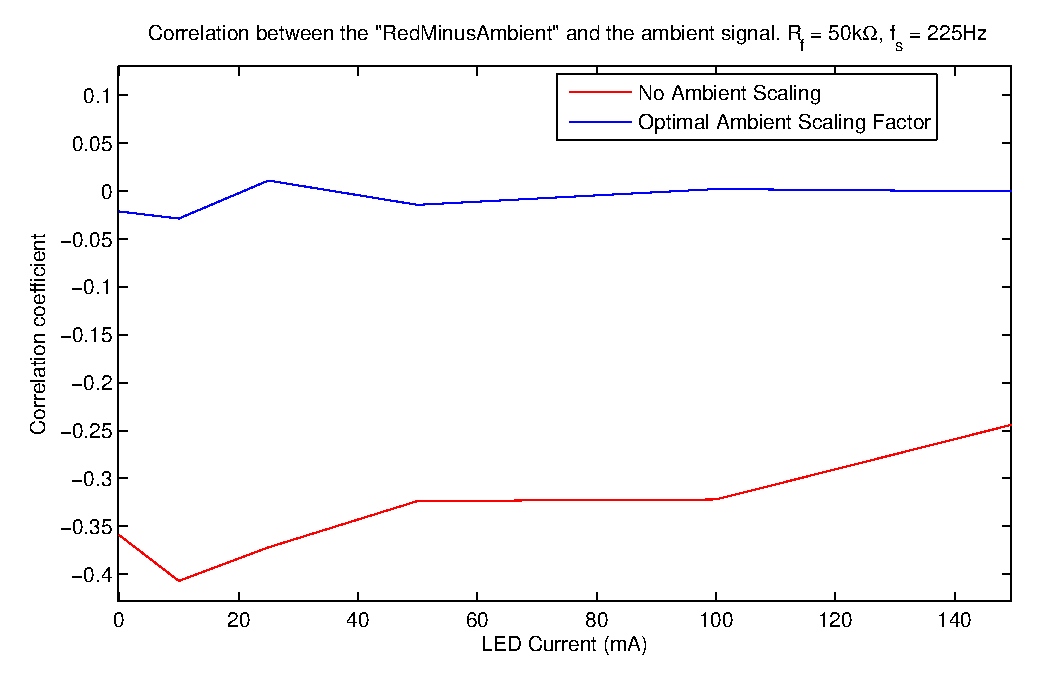
\includegraphics[scale=0.8]{kuvat/measurements/redMinusAmbient_ambient_correlation.eps}
%  \caption{The correlation between the ``Red Minus Ambient'' signal and the ambient signal when using different ambient scaling factors. The results show that with no scaling the processed signal still correlates with the original ambient one, indicating that the subtraction process doesn't perform optimally. It also shows that the result improves when using an optimal scaling factor.}
%  \label{fig:redMinusAmbient_ambient_correlation}
%\end{center}
%\end{figure}

\begin{figure}[htcb!]
\begin{center}
  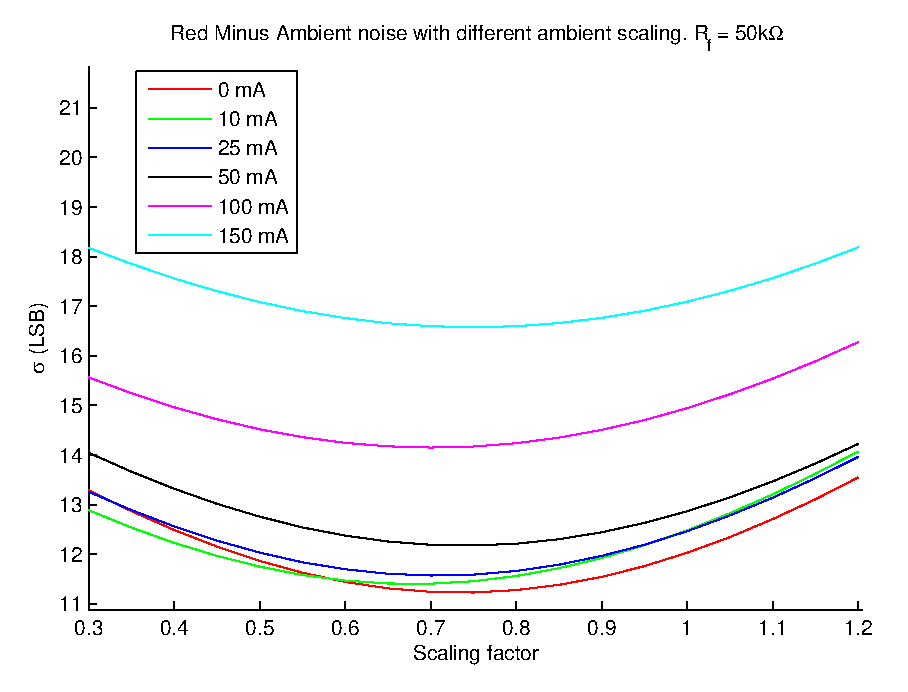
\includegraphics{kuvat/measurements/noise_vs_ambient_scaling.eps}
  \caption{The noise of the processed signal as a function of ambient scaling. The results show that the ambient channel signal path amplifies the common-mode noise significantly compared to the red channel, the noise in the processed signal having a minimum at a scaling factor around 0.7 even when measuring a zero signal.}
  \label{fig:noise_vs_ambient_scaling}
\end{center}
\end{figure}

\subsection{Conclusion of the First Testing Round}\label{section:analysis_conclusion}

The static tests showed that the new hardware has the potential to meet its specifications and they were also used to find the optimal operating parameters. On the other hand, the dynamic tests showed a significant decrease in performance when using the AFE in a normal pulsed current mode, indicating a flaw in the receiver's sampling and conversion circuitry. The data led to a conclusion that the receiver's signal chain was flawed and didn't handle a pulsed signal well. It was also concluded that said flaw would most probably be found in the buffer feeding the ADC or somewhere nearby.

The conclusion with data to support it was delivered to the hardware team which after considerable time indeed identified a defect in the buffer, proving the hypothesis true. The buffer couldn't properly handle the square-wave resulting from the subsequent conversion of signal and ambient channels; instead it added a considerable amount of noise on top of the wave but not on the bottom, resulting in that the noises in the two channels didn't correlate. Therefore when subtracting ambient the system's low frequency noise didn't cancel itself out as much as planned.

The hardware team implemented a temporary fix to test the impact of the matter. Figure \ref{fig:noise_vs_current_post_fix} shows that the fix greatly improved system performance when dealing with high signals. There still exists a linear current-noise relationship but its magnitude is significantly lower than before and could diminish even further once the fix is properly implemented.

\begin{figure}[htcb]
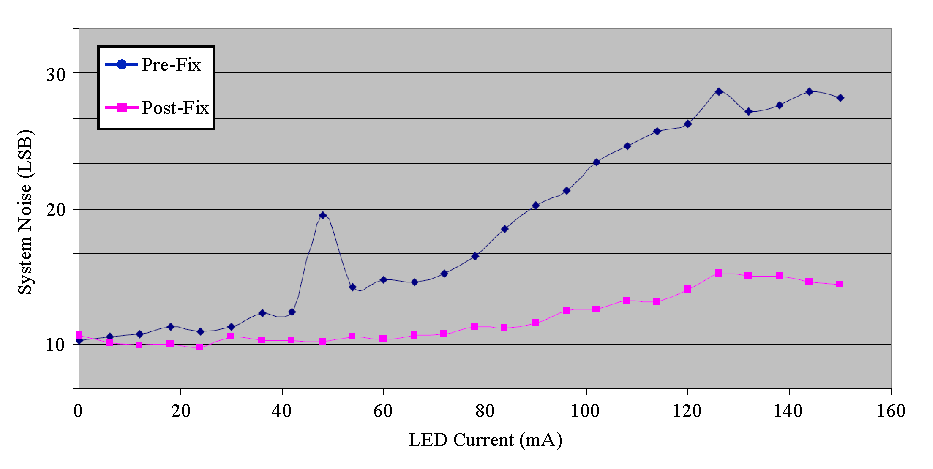
\includegraphics{kuvat/measurements/noise_vs_current_post_fix.eps}
\caption{System noise as a function of LED current before and after the temporary fix of the ADC's buffer. The results show that the fix improved the system's noise performance.}
\label{fig:noise_vs_current_post_fix}
\end{figure}

\subsection{Suitability for Low Power Applications}

After having determined that the performance of the AFE looked good enough for performance applications, it was time to decide whether the design concept as a whole suited the needs of the business. The key point in this was that in the optimal case the system would deliver a measurement good enough in all the different use cases (performance, low power, ultra-low power for wireless) with a reasonable price.


\subsubsection{Minimum Power Requirements}

The absolute minimum power the front-end can be operated with is set by the constant power consumption of the transmitter, the receiver and the microcontroller, totaling in ca.\ 6 mW. In addition to that, the system also needs power to feed the LEDs -- the general rule is that the more power is put into them the better signal-to-noise ratio is achieved, thus making the measurement more accurate. So far the absolute minimum LED power with which a typical finger can be measured is in the range of 1 mW but it only works reliably in the optimal case; typically the LEDs operate with 10-150 mW of power.

\subsubsection{Minimum Signal-to-Noise Ratio in Practice}

As explained in section \ref{section:noise_characterization}, the system needs to report the patient's \spo value with no more than 2 \%-points of error. This is interpreted so that taking into account physical variability the standard deviation of the \spo value must be less than 1 \%-point during a period of time, assuming that the mean value is static and reported correctly. In practice this means that the patient's blood perfusion has a lower limit after which the system's signal-to-noise ratio is too low for accurate measuring. Many manufacturers use a Bio-Tek \spo simulator \cite{Bio-Tek} to validate their low perfusion claims but it was found that the simulator itself produces more noise than the system to be tested as can be seen in figure \ref{fig:biotek_DC_noise}; this prompted new methods for assessing the system's limits.

\begin{figure}[htcb]
  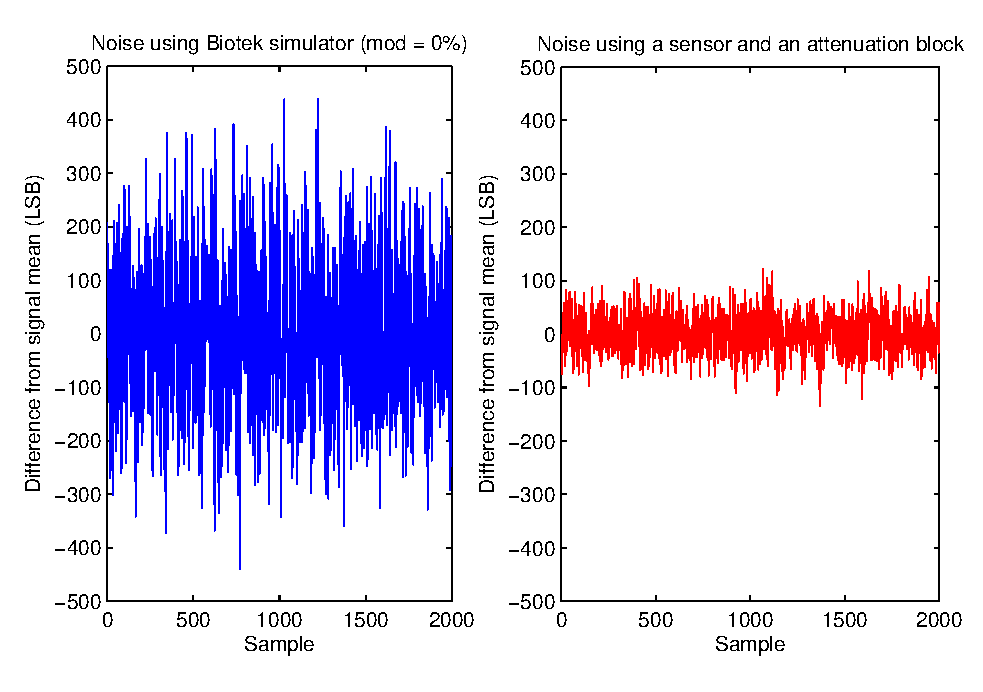
\includegraphics[scale=0.9]{kuvat/measurements/biotek_DC_noise.eps}
  \caption{The noises of two measurements with same AFE settings and signal levels, one using the Bio-Tek simulator in DC mode and one using just a light attenuation block in the sensor. It can be seen that the Bio-Tek simulator introduces a lot of noise into the system, rendering direct low perfusion performance tests pointless.}
  \label{fig:biotek_DC_noise}
\end{figure}

Having the system's theory in a good shape, the Bio-Tek simulator was used a bit differently: depending on the modulation settings the signal quality varied and subsequently the \spo algorithm provided readings of different standard deviations. The actual noise level of each of the signals was calculated by fitting an ideal simulator output signal on the data and subtracting it, leaving only noise from the simulator itself and the system. Thus it was possible to draw a relationship between system performance (or signal quality) as seen by the algorithm and \spo variability which is shown in figure \ref{fig:spo2_noise_vs_snr}. 

\begin{figure}[htcb]
	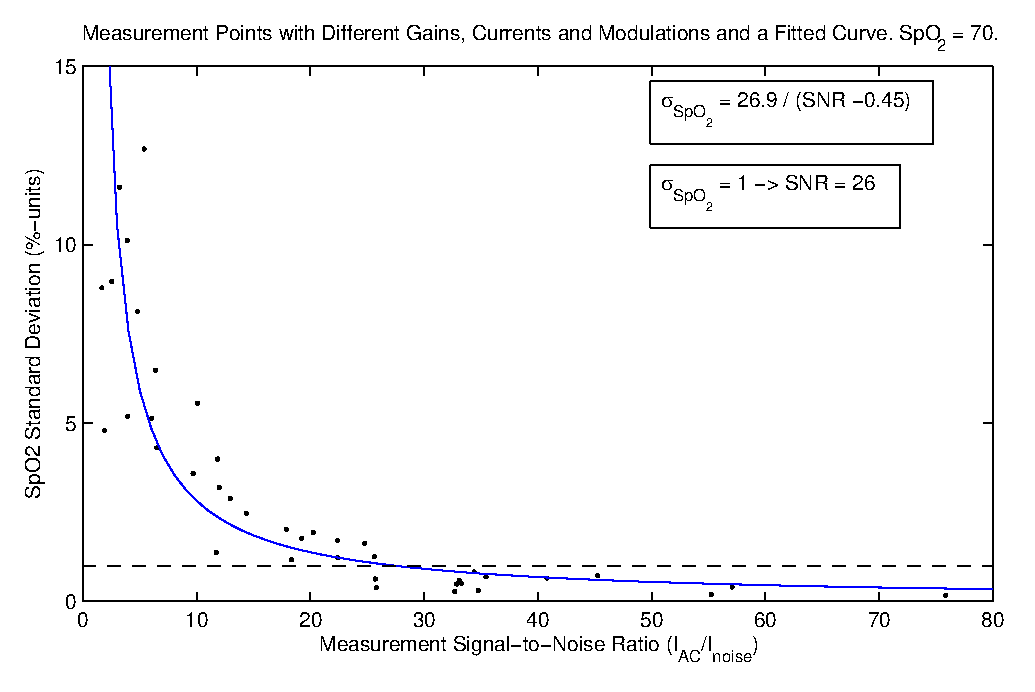
\includegraphics[scale=0.9]{kuvat/measurements/spo2_error_vs_measurement_snr.eps}
	\caption{The relationship between the effective AC signal-to-noise ratio and \spo standard deviation. A 1/SNR curve was fitted on the measurement data. The data shows that to achieve \spo standard deviation of 1 or smaller the AC peak-to-peak signal has to be at least 26 times bigger than RMS noise. For an IR modulation of 0.02\% this translates to a SNR requirement of 102 dB.}
	\label{fig:spo2_noise_vs_snr}
\end{figure}

The data clearly follows a 1/SNR type curve. From the curve it can be concluded that the IR AC signal needs to be 26 times bigger than RMS noise, or in other words the SNR\subscript{AC} has to be at least 26, to achieve an \spo standard deviation of 1 \%-point. This value was fixed to draw a relationship between system noise requirements and IR modulation as per equation (\ref{eq:noise_vs_mod}), shown in figure \ref{fig:noise_vs_mod}. Overall, for an IR modulation of 0.02\% this means that the system's total SNR has to be at least 102 dB. It's more than predicted in figure \ref{fig:noise_requirement_vs_spo2_fft} but it's to be noted that the noise isn't white when using the simulator -- due to its properties a lot of the noise is in the fundamental frequency, effectively increasing the value of $\beta$ in table \ref{tbl:specification_constants}.

\begin{equation}
  SNR_{AC} = \frac{I_{AC}}{I_n} = \frac{m_{IR} \cdot I_{DC}}{I_n} \rightarrow I_n = \frac{m_{IR} \cdot I_{DC}}{SNR_{AC}}
  \label{eq:noise_vs_mod}
\end{equation}

\begin{figure}[htcb]
	\centergraphics{kuvat/measurements/noise_vs_mod.eps}
	\caption{System maximum noise allowed for a reliable measurement as a function of IR modulation as per equation \ref{eq:noise_vs_mod}. SNR\subscript{AC} is fixed to 26.45.}
	\label{fig:noise_vs_mod}
\end{figure}

